% Setting up Beamer document class for slides
\documentclass[12pt]{beamer}

% Including essential packages for formatting, code, tables, and diagrams
\usepackage[utf8]{inputenc}
\usepackage[T1]{fontenc}
\usepackage{geometry}
\geometry{paperwidth=160mm,paperheight=90mm,margin=1cm}
\usepackage{listings}
\usepackage{xcolor}
\usepackage{booktabs}
\usepackage{array}
\usepackage{parskip}
\usepackage{enumitem}
\usepackage{tikz}
\usetikzlibrary{shapes.geometric, arrows.meta, positioning}

% Using Beamer theme for professional look
\usetheme{Madrid}
\usecolortheme{default}
\setbeamertemplate{navigation symbols}{}
\setbeamertemplate{footline}[frame number]

% Defining code listing style for various languages
\lstset{
  basicstyle=\ttfamily\footnotesize,
  breaklines=true,
  frame=single,
  keywordstyle=\color{blue}\bfseries,
  commentstyle=\color{gray}\itshape,
  stringstyle=\color{red},
  numbers=left,
  numberstyle=\tiny,
  stepnumber=1,
  showspaces=false,
  showstringspaces=false,
  tabsize=2
}

% Configuring listing styles for Java, C++, SQL, and bash
\lstdefinestyle{javastyle}{
  language=Java,
  backgroundcolor=\color{lightgray!10},
  commentstyle=\color{green!60!black},
  keywordstyle=\color{blue},
  stringstyle=\color{purple},
  basicstyle=\ttfamily\footnotesize,
  breaklines=true,
  frame=single,
  numbers=left
}
\lstdefinestyle{cppstyle}{
  language=C++,
  backgroundcolor=\color{lightgray!10},
  commentstyle=\color{green!60!black},
  keywordstyle=\color{blue},
  stringstyle=\color{purple},
  basicstyle=\ttfamily\footnotesize,
  breaklines=true,
  frame=single,
  numbers=left
}
\lstdefinestyle{sqlstyle}{
  language=SQL,
  backgroundcolor=\color{lightgray!10},
  commentstyle=\color{green!60!black},
  keywordstyle=\color{blue},
  stringstyle=\color{purple},
  basicstyle=\ttfamily\footnotesize,
  breaklines=true,
  frame=single,
  numbers=left
}
\lstdefinestyle{bashstyle}{
  language=bash,
  backgroundcolor=\color{lightgray!10},
  commentstyle=\color{green!60!black},
  keywordstyle=\color{blue},
  stringstyle=\color{purple},
  basicstyle=\ttfamily\footnotesize,
  breaklines=true,
  frame=single,
  numbers=left
}

% Defining TikZ styles for diagrams
\tikzset{
  box/.style={rectangle, draw, rounded corners, minimum height=2em, minimum width=4em, align=center},
  arrow/.style={-Stealth, thick},
}

% Loading font package last for compatibility
\usepackage{noto}

% Title slide information
\title{Secure Software Design and Development Training}
\subtitle{Protecting Sensitive Data for NADRA}
\author{Muhammad Ahmad Nawaz}
\institute{National Database \& Registration Authority (NADRA)}
\date{August 2025}

% Beginning the document
\begin{document}

% Title slide
\begin{frame}
  \titlepage
\end{frame}

% Agenda slide
\begin{frame}{Agenda}
  \begin{enumerate}
    \item Introduction to Secure Software Design
    \item Avoiding Hardcoded Credentials
    \item Preventing Memory Safety Issues
    \item Handling Integer Overflows and Underflows
    \item Ensuring Safe Memory Usage
    \item Web and Authentication Security
    \item Analysis Tools and Best Practices
    \item Summary and Resources
  \end{enumerate}
\end{frame}

% Introduction to Secure Software Design
\begin{frame}{Introduction to Secure Software Design}
  \begin{block}{Why It Matters for NADRA}
    \begin{itemize}
      \item Manages biometric and demographic data of 120M+ citizens
      \item Critical national infrastructure with global connections
      \item High-value target for threat actors
      \item Must comply with GDPR, ISO 27001, and national laws
    \end{itemize}
  \end{block}
  \begin{alertblock}{Key Principle}
    Security is a \textbf{fundamental requirement}, not an add-on.
  \end{alertblock}
  % Visual: NADRA's data flow diagram
  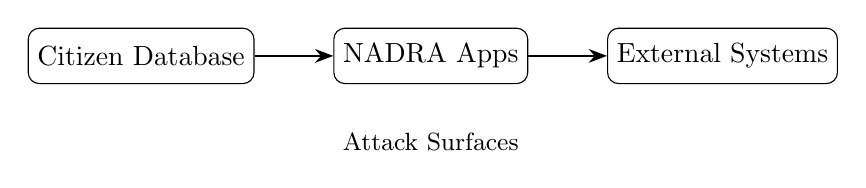
\begin{tikzpicture}
    \node[box] (db) {Citizen Database};
    \node[box, right=of db] (app) {NADRA Apps};
    \node[box, right=of app] (external) {External Systems};
    \draw[arrow] (db) -- (app);
    \draw[arrow] (app) -- (external);
    \node[below=0.5cm of app] {\small Attack Surfaces};
  \end{tikzpicture}
\end{frame}

% Core Security Principles
\begin{frame}{Core Security Principles}
  \begin{description}
    \item[Defense in Depth] Multiple security layers.
    \item[Least Privilege] Minimum necessary permissions.
    \item[Secure by Default] Systems secure out of the box.
    \item[Fail Securely] Secure state on failure.
  \end{description}
  % Visual: Layered security model
  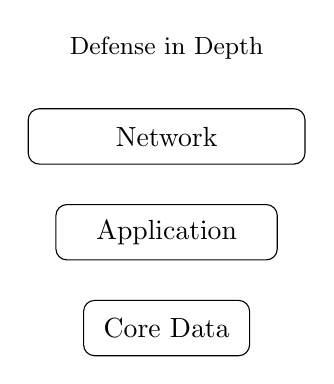
\begin{tikzpicture}
    \node[box, minimum width=6em] (core) {Core Data};
    \node[box, minimum width=8em, above=0.5cm of core] (app) {Application};
    \node[box, minimum width=10em, above=0.5cm of app] (network) {Network};
    \node[above=0.5cm of network] {\small Defense in Depth};
  \end{tikzpicture}
\end{frame}

% Hardcoded Credentials: Risks
\begin{frame}{Hardcoded Credentials: Risks}
  \begin{block}{What Are They?}
    Passwords, API keys, or secrets embedded in source code.
  \end{block}
  \begin{alertblock}{Risks for NADRA}
    \begin{itemize}
      \item Exposure via code leaks or decompilation
      \item Hard to rotate credentials
      \item Violates GDPR, ISO 27001
      \item Risks biometric data exposure
    \end{itemize}
  \end{alertblock}
  % Visual: Code leak exposure diagram
  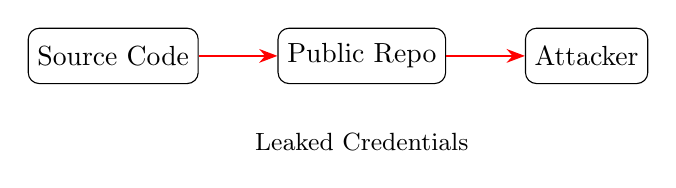
\begin{tikzpicture}
    \node[box] (code) {Source Code};
    \node[box, right=of code] (repo) {Public Repo};
    \node[box, right=of repo] (attacker) {Attacker};
    \draw[arrow, red] (code) -- (repo);
    \draw[arrow, red] (repo) -- (attacker);
    \node[below=0.5cm of repo] {\small Leaked Credentials};
  \end{tikzpicture}
\end{frame}

% Hardcoded Credentials: Vulnerable Example
\begin{frame}[fragile]{Hardcoded Credentials: Vulnerable Example}
  \begin{lstlisting}[style=javastyle]
public class DatabaseConnector {
    public Connection getConnection() {
        String url = "jdbc:mysql://db.nadra.gov";
        String username = "admin"; // Hardcoded!
        String password = "Nadra@123"; // Hardcoded!
        return DriverManager.getConnection(url, username, password);
    }
}
  \end{lstlisting}
  \begin{alertblock}{Vulnerability}
    Exposed credentials risk unauthorized access to NADRA’s citizen database.
  \end{alertblock}
\end{frame}

% Hardcoded Credentials: Secure Alternatives
\begin{frame}[fragile]{Hardcoded Credentials: Secure Alternatives}
  \begin{block}{Best Practices}
    \begin{itemize}
      \item \textbf{Environment Variables}:
        \begin{lstlisting}[style=javastyle]
spring.datasource.url=${DB_URL}
spring.datasource.username=${DB_USERNAME}
spring.datasource.password=${DB_PASSWORD}
        \end{lstlisting}
      \item \textbf{Secrets Management}: Use HashiCorp Vault or AWS Secrets Manager.
      \item \textbf{IAM Roles}: Credential-less access for NADRA services.
    \end{itemize}
  \end{block}
  % Visual: Secrets management workflow
  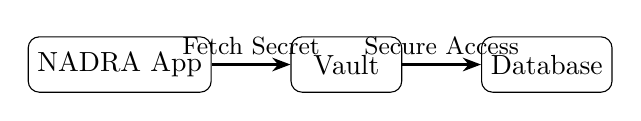
\begin{tikzpicture}
    \node[box] (app) {NADRA App};
    \node[box, right=of app] (vault) {Vault};
    \node[box, right=of vault] (db) {Database};
    \draw[arrow] (app) -- (vault) node[midway, above] {\small Fetch Secret};
    \draw[arrow] (vault) -- (db) node[midway, above] {\small Secure Access};
  \end{tikzpicture}
\end{frame}

% Secrets Management Best Practices
\begin{frame}{Secrets Management Best Practices}
  \begin{itemize}
    \item \textbf{Regular Rotation}: Automate credential updates.
    \item \textbf{Encryption}: Secure at rest and in transit.
    \item \textbf{Access Control}: Role-based access for NADRA staff.
    \item \textbf{Audit Trails}: Log all credential access for compliance.
  \end{itemize}
  % Visual: Credential lifecycle
  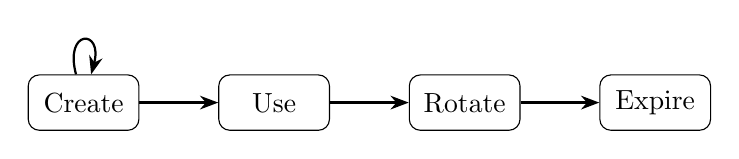
\begin{tikzpicture}
    \node[box] (create) {Create};
    \node[box, right=of create] (use) {Use};
    \node[box, right=of use] (rotate) {Rotate};
    \node[box, right=of rotate] (expire) {Expire};
    \draw[arrow, loop above] (create) to (create);
    \draw[arrow] (create) -- (use);
    \draw[arrow] (use) -- (rotate);
    \draw[arrow] (rotate) -- (expire);
  \end{tikzpicture}
\end{frame}

% Memory Safety: Introduction
\begin{frame}{Memory Safety: Introduction}
  \begin{block}{What Is Memory Safety?}
    Preventing vulnerabilities from improper memory handling (e.g., buffer overflows, use-after-free).
  \end{block}
  \begin{alertblock}{Impact}
    Memory issues cause \textasciitilde70\% of vulnerabilities in C/C++ software.
  \end{alertblock}
  % Visual: Vulnerability prevalence chart
  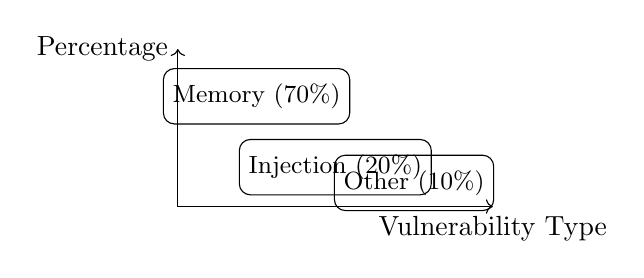
\begin{tikzpicture}
    \draw[->] (0,0) -- (4,0) node[below] {Vulnerability Type};
    \draw[->] (0,0) -- (0,2) node[left] {Percentage};
    \node[box, minimum width=1cm] at (1,1.4) {\small Memory (70\%)};
    \node[box, minimum width=1cm] at (2,0.5) {\small Injection (20\%)};
    \node[box, minimum width=1cm] at (3,0.3) {\small Other (10\%)};
  \end{tikzpicture}
\end{frame}

% Buffer Overflow: Vulnerable Example
\begin{frame}[fragile]{Buffer Overflow: Vulnerable Example}
  \begin{lstlisting}[style=cppstyle]
void process_input(char* input) {
    char buffer[16]; // Only 16 bytes
    strcpy(buffer, input); // No bounds checking!
    printf("Input processed: %s\n", buffer);
}
  \end{lstlisting}
  \begin{alertblock}{Vulnerability}
    Overflows can overwrite stack, enabling code execution or crashes.
  \end{alertblock}
  % Visual: Stack overflow attack
  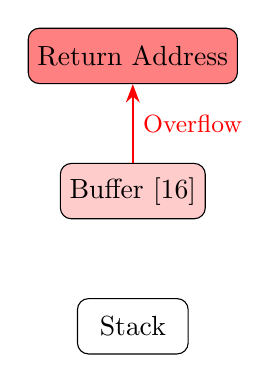
\begin{tikzpicture}
    \node[box] (stack) {Stack};
    \node[box, above=of stack, fill=red!20] (buffer) {Buffer [16]};
    \node[box, above=of buffer, fill=red!50] (return) {Return Address};
    \draw[arrow, red] (buffer) -- (return) node[midway, right] {\small Overflow};
  \end{tikzpicture}
\end{frame}

% Buffer Overflow: Secure Example
\begin{frame}[fragile]{Buffer Overflow: Secure Example}
  \begin{lstlisting}[style=cppstyle]
void process_input(char* input) {
    char buffer[16];
    strncpy(buffer, input, sizeof(buffer) - 1);
    buffer[sizeof(buffer) - 1] = '\0';
    printf("Input processed: %s\n", buffer);
}
  \end{lstlisting}
  \begin{block}{Prevention}
    \begin{itemize}
      \item Use \texttt{strncpy}, \texttt{snprintf} for bounds checking.
      \item Validate input length.
      \item Enable ASLR, DEP, stack canaries.
    \end{itemize}
  \end{block}
\end{frame}

% Buffer Overflow in Java/JNI
\begin{frame}[fragile]{Buffer Overflow in Java/JNI}
  \begin{lstlisting}[style=javastyle]
public class NativeProcessor {
    static { System.loadLibrary("processor"); }
    public native void processData(byte[] data);
    public void handleUserInput(String input) {
        byte[] data = input.getBytes();
        processData(data); // No validation
    }
}
  \end{lstlisting}
  \begin{lstlisting}[style=cppstyle]
JNIEXPORT void JNICALL Java_NativeProcessor_processData(
    JNIEnv *env, jobject obj, jbyteArray data) {
    jbyte *buffer = (*env)->GetByteArrayElements(env, data, NULL);
    jsize length = (*env)->GetArrayLength(env, data);
    char localBuffer[128];
    memcpy(localBuffer, buffer, length); // Overflow risk
}
  \end{lstlisting}
  % Visual: JNI memory layout
  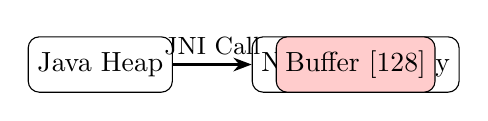
\begin{tikzpicture}
    \node[box] (java) {Java Heap};
    \node[box, right=of java] (native) {Native Memory};
    \node[box, fill=red!20] at (native) {Buffer [128]};
    \draw[arrow] (java) -- (native) node[midway, above] {\small JNI Call};
  \end{tikzpicture}
\end{frame}

% Use-After-Free: Vulnerable Example
\begin{frame}[fragile]{Use-After-Free: Vulnerable Example}
  \begin{lstlisting}[style=cppstyle]
void processUser() {
    User* user = new User();
    strcpy(user->name, "guest");
    user->isAdmin = false;
    delete user; // Freed
    if (user->isAdmin) { // Use after free
        grantAdminAccess();
    }
}
  \end{lstlisting}
  \begin{alertblock}{Impact}
    Can lead to privilege escalation or crashes.
  \end{alertblock}
  % Visual: Use-after-free memory corruption
  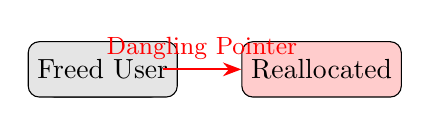
\begin{tikzpicture}
    \node[box] (mem) {Memory};
    \node[box, fill=gray!20] at (mem) {Freed User};
    \node[box, right=of mem, fill=red!20] (reallocated) {Reallocated};
    \draw[arrow, red] (mem) -- (reallocated) node[midway, above] {\small Dangling Pointer};
  \end{tikzpicture}
\end{frame}

% Use-After-Free: Secure Example
\begin{frame}[fragile]{Use-After-Free: Secure Example}
  \begin{lstlisting}[style=cppstyle]
void processUser() {
    std::unique_ptr<User> user = std::make_unique<User>();
    strcpy(user->name, "guest");
    user->isAdmin = false;
    user.reset(); // Auto-deleted
}
  \end{lstlisting}
  \begin{block}{Prevention}
    \begin{itemize}
      \item Use \texttt{std::unique_ptr}, \texttt{std::shared_ptr}.
      \item Nullify pointers after \texttt{delete}.
      \item Prefer memory-safe languages (Java, Rust).
    \end{itemize}
  \end{block}
\end{frame}

% Integer Overflow: Vulnerable Example
\begin{frame}[fragile]{Integer Overflow: Vulnerable Example}
  \begin{lstlisting}[style=cppstyle]
void allocate_buffer(size_t user_size) {
    size_t buffer_size = user_size + 20; // Overflow risk
    if (buffer_size < MAX_ALLOCATION) {
        char* buffer = (char*)malloc(buffer_size);
        // Use buffer...
    }
}
  \end{lstlisting}
  \begin{alertblock}{Impact}
    Wraparound leads to small buffer, causing overflow.
  \end{alertblock}
  % Visual: Integer overflow wraparound
  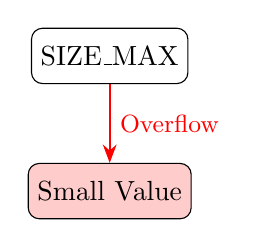
\begin{tikzpicture}
    \node[box] (max) {SIZE\_MAX};
    \node[box, below=of max, fill=red!20] (small) {Small Value};
    \draw[arrow, red] (max) -- (small) node[midway, right] {\small Overflow};
  \end{tikzpicture}
\end{frame}

% Integer Overflow: Secure Example
\begin{frame}[fragile]{Integer Overflow: Secure Example}
  \begin{lstlisting}[style=cppstyle]
void allocate_buffer(size_t user_size) {
    if (user_size > SIZE_MAX - 20) {
        return; // Prevent overflow
    }
    size_t buffer_size = user_size + 20;
    if (buffer_size < MAX_ALLOCATION) {
        char* buffer = (char*)malloc(buffer_size);
        // Use buffer...
    }
}
  \end{lstlisting}
  \begin{block}{Prevention}
    \begin{itemize}
      \item Check arithmetic bounds.
      \item Use safe integer libraries.
      \item Enable \texttt{-ftrapv} compiler flag.
    \end{itemize}
  \end{block}
\end{frame}

% Integer Underflow in Java
\begin{frame}[fragile]{Integer Underflow in Java}
  \begin{lstlisting}[style=javastyle]
public void processData(int count, int headerSize) {
    int dataSize = count - headerSize; // Underflow risk
    byte[] buffer = new byte[dataSize]; // Throws exception
}
  \end{lstlisting}
  \begin{lstlisting}[style=javastyle]
public void processData(int count, int headerSize) {
    if (count < headerSize) {
        throw new IllegalArgumentException("Count too small");
    }
    int dataSize = Math.subtractExact(count, headerSize);
    byte[] buffer = new byte[dataSize];
}
  \end{lstlisting}
  % Visual: Exception handling flow
  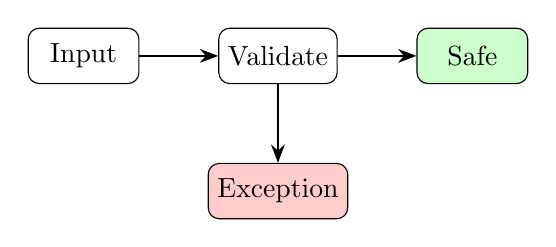
\begin{tikzpicture}
    \node[box] (input) {Input};
    \node[box, right=of input] (validate) {Validate};
    \node[box, right=of validate, fill=green!20] (safe) {Safe};
    \node[box, below=of validate, fill=red!20] (exception) {Exception};
    \draw[arrow] (input) -- (validate);
    \draw[arrow] (validate) -- (safe);
    \draw[arrow] (validate) -- (exception);
  \end{tikzpicture}
\end{frame}

% Safe Memory Usage in Java
\begin{frame}[fragile]{Safe Memory Usage in Java}
  \begin{lstlisting}[style=javastyle]
@Service
public class FileService {
    public String readFile(String path) {
        try (BufferedReader reader = new BufferedReader(
                new FileReader(path))) {
            StringBuilder content = new StringBuilder();
            String line;
            while ((line = reader.readLine()) != null) {
                content.append(line).append("\n");
            }
            return content.toString();
        } catch (IOException e) {
            throw new RuntimeException("File error", e);
        }
    }
}
  \end{lstlisting}
  \begin{block}{Best Practices}
    \begin{itemize}
      \item Use \texttt{try-with-resources}.
      \item Validate sizes before allocation.
      \item Limit direct memory access.
    \end{itemize}
  \end{block}
\end{frame}

% Web Security: SQL Injection
\begin{frame}[fragile]{Web Security: SQL Injection}
  \begin{lstlisting}[style=javastyle]
@Repository
public class UserDao {
    @Autowired private JdbcTemplate jdbcTemplate;
    // Vulnerable
    public User findByUsername(String username) {
        String sql = "SELECT * FROM users WHERE username = '" + username + "'";
        return jdbcTemplate.queryForObject(sql, new UserRowMapper());
    }
    // Secure
    public User findByUsername(String username) {
        String sql = "SELECT * FROM users WHERE username = ?";
        return jdbcTemplate.queryForObject(sql, new UserRowMapper(), username);
    }
}
  \end{lstlisting}
  % Visual: SQL injection attack
  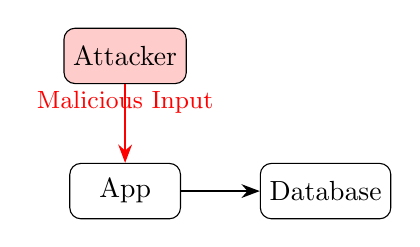
\begin{tikzpicture}
    \node[box] (app) {App};
    \node[box, right=of app] (db) {Database};
    \node[box, above=of app, fill=red!20] (attacker) {Attacker};
    \draw[arrow, red] (attacker) -- (app) node[midway, above] {\small Malicious Input};
    \draw[arrow] (app) -- (db);
  \end{tikzpicture}
\end{frame}

% Web Security: XSS Prevention
\begin{frame}[fragile]{Web Security: XSS Prevention}
  \begin{lstlisting}[style=javastyle]
@Controller
public class ProfileController {
    // Vulnerable
    public String showProfile(Model model, @RequestParam String name) {
        model.addAttribute("welcomeMessage", "Welcome, " + name);
        return "profile";
    }
    // Secure
    public String showProfile(Model model, @RequestParam String name) {
        if (!isValidName(name)) {
            throw new IllegalArgumentException("Invalid name");
        }
        model.addAttribute("welcomeMessage", "Welcome, " + name);
        return "profile";
    }
}
  \end{lstlisting}
  % Visual: XSS attack flow
  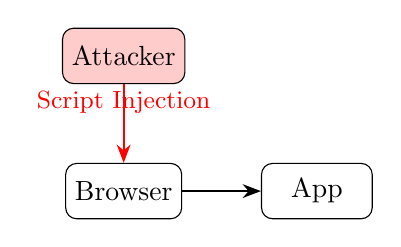
\begin{tikzpicture}
    \node[box] (browser) {Browser};
    \node[box, right=of browser] (app) {App};
    \node[box, above=of browser, fill=red!20] (attacker) {Attacker};
    \draw[arrow, red] (attacker) -- (browser) node[midway, above] {\small Script Injection};
    \draw[arrow] (browser) -- (app);
  \end{tikzpicture}
\end{frame}

% Authentication Best Practices
\begin{frame}[fragile]{Authentication Best Practices}
  \begin{lstlisting}[style=javastyle]
@Bean
public PasswordEncoder passwordEncoder() {
    return new BCryptPasswordEncoder(12);
}
@Service
public class LoginAttemptService {
    private final int MAX_ATTEMPT = 5;
    private LoadingCache<String, Integer> attemptsCache;
    // Track and lockout failed attempts
}
  \end{lstlisting}
  \begin{block}{Key Practices}
    \begin{itemize}
      \item Use \texttt{BCrypt} for password hashing.
      \item Implement multi-factor authentication (MFA).
      \item Enforce account lockout.
    \end{itemize}
  \end{block}
\end{frame}

% Authentication Attack Vectors
\begin{frame}{Authentication Attack Vectors}
  \begin{block}{Frequency of Attacks}
    \begin{tabular}{|l|c|}
      \hline
      \textbf{Attack Type} & \textbf{Frequency (\%)} \\ \hline
      Brute Force & 40\% \\ \hline
      Credential Stuffing & 30\% \\ \hline
      Phishing & 20\% \\ \hline
      Session Hijacking & 10\% \\ \hline
    \end{tabular}
  \end{block}
  % Visual: Attack vector chart
  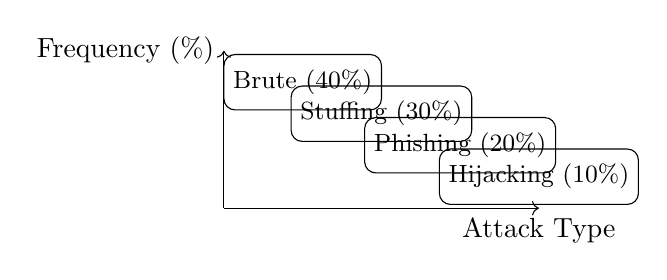
\begin{tikzpicture}
    \draw[->] (0,0) -- (4,0) node[below] {Attack Type};
    \draw[->] (0,0) -- (0,2) node[left] {Frequency (\%)};
    \node[box, minimum width=1cm] at (1,1.6) {\small Brute (40\%)};
    \node[box, minimum width=1cm] at (2,1.2) {\small Stuffing (30\%)};
    \node[box, minimum width=1cm] at (3,0.8) {\small Phishing (20\%)};
    \node[box, minimum width=1cm] at (4,0.4) {\small Hijacking (10\%)};
  \end{tikzpicture}
\end{frame}

% Role-Based Access Control (RBAC)
\begin{frame}[fragile]{Role-Based Access Control (RBAC)}
  \begin{lstlisting}[style=javastyle]
@Configuration
@EnableWebSecurity
public class SecurityConfig extends WebSecurityConfigurerAdapter {
    @Override
    protected void configure(HttpSecurity http) throws Exception {
        http.authorizeRequests()
            .antMatchers("/api/admin/**").hasRole("ADMIN")
            .antMatchers("/api/user/**").hasAnyRole("USER", "ADMIN")
            .anyRequest().authenticated();
    }
}
  \end{lstlisting}
  % Visual: RBAC hierarchy
  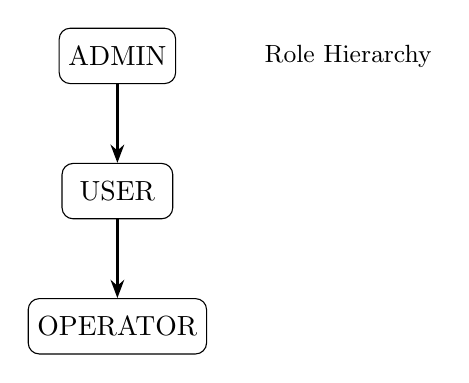
\begin{tikzpicture}
    \node[box] (admin) {ADMIN};
    \node[box, below=of admin] (user) {USER};
    \node[box, below=of user] (operator) {OPERATOR};
    \draw[arrow] (admin) -- (user);
    \draw[arrow] (user) -- (operator);
    \node[right=of admin] {\small Role Hierarchy};
  \end{tikzpicture}
\end{frame}

% Analysis Tools
\begin{frame}{Analysis Tools}
  \begin{block}{Static Analysis}
    \begin{itemize}
      \item \textbf{Coverity}: Complex defect detection.
      \item \textbf{SonarQube}: Security vulnerabilities, code smells.
      \item \textbf{Clang}: C/C++ memory issues.
    \end{itemize}
  \end{block}
  \begin{block}{Dynamic Analysis}
    \begin{itemize}
      \item \textbf{AddressSanitizer}: Memory errors.
      \item \textbf{Valgrind}: Memory and threading bugs.
      \item \textbf{OWASP ZAP}: Web vulnerabilities.
    \end{itemize}
  \end{block}
  % Visual: Tool comparison
  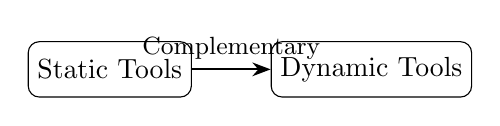
\begin{tikzpicture}
    \node[box] (static) {Static Tools};
    \node[box, right=of static] (dynamic) {Dynamic Tools};
    \draw[arrow] (static) -- (dynamic) node[midway, above] {\small Complementary};
  \end{tikzpicture}
\end{frame}

% Secure Coding Practices
\begin{frame}{Secure Coding Practices}
  \begin{itemize}
    \item \textbf{Input Validation}: Check type, length, format, range.
    \item \textbf{Output Encoding}: Prevent XSS with proper encoding.
    \item \textbf{Least Privilege}: Minimize permissions.
    \item \textbf{Defense in Depth}: Multiple security layers.
    \item \textbf{Secure Error Handling}: Avoid sensitive data leaks.
  \end{itemize}
  % Visual: Secure coding workflow
  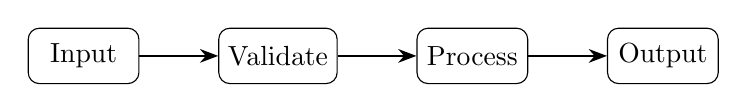
\begin{tikzpicture}
    \node[box] (input) {Input};
    \node[box, right=of input] (validate) {Validate};
    \node[box, right=of validate] (process) {Process};
    \node[box, right=of process] (output) {Output};
    \draw[arrow] (input) -- (validate);
    \draw[arrow] (validate) -- (process);
    \draw[arrow] (process) -- (output);
  \end{tikzpicture}
\end{frame}

% Summary
\begin{frame}{Summary}
  \begin{block}{Key Takeaways}
    \begin{itemize}
      \item Avoid hardcoded credentials with secrets management.
      \item Prevent memory issues (buffer overflows, use-after-free).
      \item Handle integer operations safely.
      \item Use static/dynamic analysis tools.
      \item Build security into every development phase.
    \end{itemize}
  \end{block}
  % Visual: Summary infographic
  \begin{tikzpicture}
    \node[box, minimum height=3cm, minimum width=6cm] (summary) {
      \begin{itemize}
        \item Secure Credentials
        \item Memory Safety
        \item Safe Arithmetic
        \item Analysis Tools
      \end{itemize}
    };
    \node[above=of summary] {\small Key Security Areas};
  \end{tikzpicture}
\end{frame}

% Resources and References
\begin{frame}{Resources \& References}
  \begin{block}{Standards}
    \begin{itemize}
      \item OWASP Secure Coding Practices
      \item CERT Secure Coding Standards
      \item CWE/SANS Top 25 Errors
    \end{itemize}
  \end{block}
  \begin{block}{Books}
    \begin{itemize}
      \item ``Secure Coding in C and C++'' by Robert C. Seacord
      \item ``The Art of Software Security Assessment'' by Mark Dowd
    \end{itemize}
  \end{block}
  \begin{block}{Contact}
    Engr.ahmad.Nawaz@giki.edu.pk
  \end{block}
\end{frame}

% Thank You Slide
\begin{frame}{Thank You!}
  \begin{block}{Contact NADRA Security Team}
    \begin{itemize}
      \item Email: security-team@nadra.gov.pk
      \item Website: security.nadra.gov.pk
      \item Phone: +92-51-1234567
    \end{itemize}
  \end{block}
  % Visual: NADRA logo
  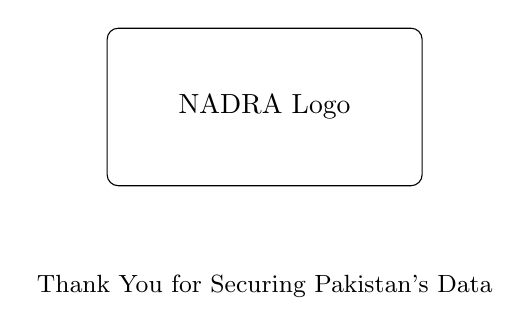
\begin{tikzpicture}
    \node[box, minimum height=2cm, minimum width=4cm] (logo) {NADRA Logo};
    \node[below=of logo] {\small Thank You for Securing Pakistan's Data};
  \end{tikzpicture}
\end{frame}

% Ending the document
\end{document}